\documentclass[a4paper, twocolumn, html, DIV=12]{scrartcl}

\usepackage[T1]{fontenc}
\usepackage[utf8]{inputenc}
\usepackage[british]{babel}

\addtokomafont{disposition}{\rmfamily}
\addtokomafont{descriptionlabel}{\rmfamily}

\usepackage{amsmath}
\usepackage{amssymb}

\usepackage{todonotes}

\usepackage{booktabs}
\usepackage{hyperref}

%\usepackage[pdftitle={Implementation of iPMCMC in Monad-Bayes},
  %pdfauthor={Per Engström},
  %pdffitwindow=true,
  %breaklinks=true,
  %colorlinks=true,
  %urlcolor=blue,
  %linkcolor=red,
  %citecolor=red,
  %anchorcolor=red]{hyperref}
%\usepackage{pdfpages}
%\usepackage{algorithm}
%\usepackage{algorithmic}
%\usepackage{natbib}


\usepackage[]{minted}
\usemintedstyle{solarizedlight}
\usepackage{mdframed}
\surroundwithmdframed{minted}


\usepackage{tikz}
\usetikzlibrary{positioning,backgrounds,matrix}
\definecolor{sbase03}{HTML}{002B36}


\title{Interacting Particle Inference for Probabilistic Programing in Haskell}

\author{Per Engström}

\date{\today}

\begin{document}
\twocolumn[
  \begin{@twocolumnfalse}
    \maketitle
    \begin{abstract}
Probabilistic programming shows much promise as a declarative way to define statistical models, but inference is often expensive. A parallelisable particle MMCMC sampler is implemeted in Haskell and the DSL Monad-Bayes. The method shows good performace compared to a single SMC sampler, but the full potential of the method could not be manifested.
    \end{abstract}
  \end{@twocolumnfalse}
]


\section{Introduction}

This thesis presents a Haskell implementation of the iPMCMC sampler for Bayesian inference in the probabilistic programming DSL Monad-Bayes.

\subsection{Background}

\subsubsection{Probabilistic programming}
\label{sec:pprog}

This paradigm leverages the expressiveness and familiarity of programming
languages  to define statistical models. In addition, separating models from inference allows the models to be composable.

Central to all probabilistic languages is the ability to construct more
complex models using simpler building blocks, usually primitive distributions
and use Bayesian filtering. Consider the problem of rolling two dice and reading the result of
the first die \emph{given that the sum is larger than 5}. The outcome of a die is
assumed to be uniformly 1 through 6.
In the Monad-Bayes DSL (see section~\ref{sec:mbayes}) this may be
expressed as
\begin{minted}{Haskell}
dice :: MonadInfer m => m Int
dice = do
  a <- uniformD [1..6]
  b <- uniformD [1..6]
  condition (a + b > 7)
  return a
\end{minted}
which is very close to the actual problem description. Since the model is
discrete we may enumerate all possibilities and get the exact distribution at
the cost of exponential complexity.

\begin{center}
  
  \begin{tabular}{crrrrrr}
    \toprule
    \midrule
    $a$ & $\Pr(a)$ \\
    \midrule
    1&0.00 \\
2&0.07 \\
3&0.13\\
4&0.20 \\
5&0.27\\
6&0.33\\
\midrule
\bottomrule
  \end{tabular}
\end{center}
This thesis will focus on more efficient but approximative sampling-based
methods.

In the design of a probabilistic language the main trade-off is between
expressiveness and performance of inference. A restricted language like
BUGS~\cite{bugs} makes the inference simpler. In Universal
(Turing-complete) languages like Anglican~\cite{anglican} and
Monad-Bayes~\cite{mbayes} the inference is more challenging.

\subsubsection{Bayesian inference}

The distributions of stochastic models are often complicated and analytically
intractable. To efficiently approximate the distribution of such models several
methods have been proposed in literature. This paper focuses on sampling-based
methods of the Markov Chain Monte Carlo (MCMC) kind~\cite{mcmc}, in particular sequential
methods based on importance sampling (SMC)~\cite{smcgordon,smcdoucet} suitable
for probabilistic programs~\cite{wood}.



\section{Theory}

This section contains the necessary theory behind inference and probabilistic programs as well as details how the Monad-Bayes library works and a description of the iPMCMC method.

\subsection{Inference on probabilistic programs}
\label{sub:inference_on_probabilistic_programs}

\begin{figure}[h!]
\begin{center}
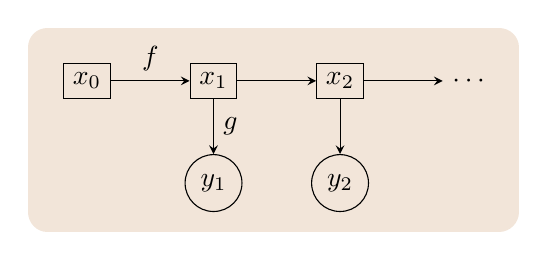
\begin{tikzpicture}[scale=1, transform shape]
    \node[draw] (x0) {$x_0$};
    \node[draw, right=of x0] (x1) {$x_1$};
    \node[draw, right=of x1] (x2) {$x_2$};
    \node[right=of x2] (x3) {$\cdots$};

    \node[draw, circle, below=2em of x1] (y1) {$y_1$};
    \node[draw, circle, below=2em of x2] (y2) {$y_2$};

    \path[-stealth]
    (x0) edge node[above] {$f$} (x1)
    (x1) edge  (x2)
    (x2) edge  (x3)
    (x1) edge node[right] {$g$} (y1)
    (x2) edge  (y2);

    \begin{pgfonlayer}{background}
        \filldraw [line width=5mm,join=round,brown!20] (x0.north west) ++ (-2mm,2mm) rectangle
        (y2.south -| x3.east);
    \end{pgfonlayer}
\end{tikzpicture}
\end{center}
\caption{A diagram of a hidden markov process.}
\label{fig:hmm}
\end{figure}

The MCMC methods are based on hidden Markov models. This is a construct of some hidden state $x_t$ evolving by some known process $f(x_t \mid x_{t-1})$ and $\mu(x_0)$ where both functions should be seen as distributions. In other words, the value of $x_t$ is not known, but the underlying process is. In addition some observations $y_t$ \emph{are} known together with their emission process $g(y_t \mid x_t)$. By comparing the measured values $y_t$ with their distribution $g$ and proposed hidden values $x_t$ it is possible to score the proposals and use the scores $w_t$ to find the most likely values.

\begin{figure}[h!]
\begin{center}
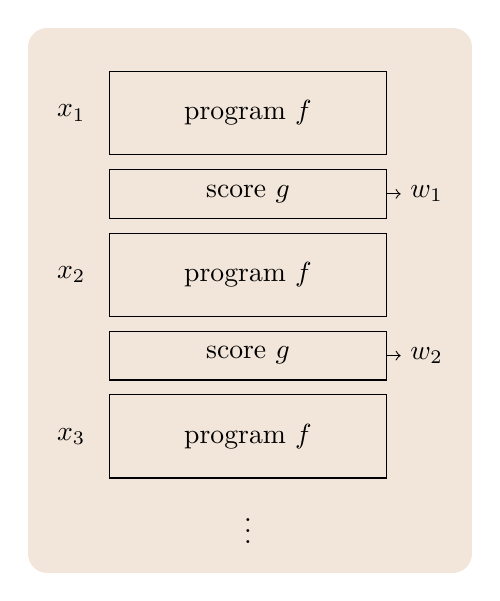
\begin{tikzpicture}[scale=1, transform shape,node distance=0.5em]
    \node[minimum width=10em,minimum height=3em,draw] (x1) {program $f$};
    \node[minimum width=10em,draw,below=of x1,inner sep=2mm] (y1) {score $g$};
    \node[minimum width=10em,minimum height=3em,draw,below=of y1] (x2) {program $f$};
    \node[minimum width=10em,draw,below=of x2,inner sep=2mm] (y2) {score $g$};
    \node[minimum width=10em,minimum height=3em,draw,below=of y2] (x3) {program $f$};

    \node[left=of x1] {$x_1$};
    \node[left=of x2] {$x_2$};
    \node[left=of x3] (xx3) {$x_3$};

    \node[right= of y1] (w1) {$w_1$};
    \node[right= of y2] (w2) {$w_2$};

    \node[below=of x3] (dots) {$\vdots$};

    \path[->]
    (y1) edge (w1)
    (y2) edge (w2);

    \begin{pgfonlayer}{background}
        \filldraw [line width=5mm,join=round,brown!20] (x1.north -| w1.east) ++ (0,3mm) rectangle
        (dots.south -| xx3.west);
    \end{pgfonlayer}
\end{tikzpicture}
\end{center}
\caption{A program seen as a hidden Markov model.}
\label{fig:hmmprog}
\end{figure}


In the context of models expressed as probabilistic programs the time aspect is more accurately viewed as the execution of the program. As the program executes random variables are sampled and combined. This corresponds to $f$ above. The program is interrupted at various points by scoring the current execution path, possibly depending on the sampled values. This is the scoring and the method for determining the score is model-dependent on $g$. These scorings separates the programs into parts, the $x_t$'s.

\subsubsection{SMC and CSMC}
\label{ssub:smc_and_csmc}



\begin{figure}[h]
\begin{center}
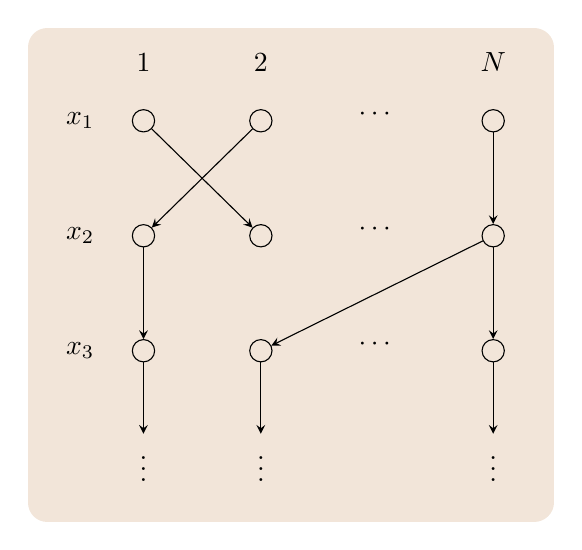
\begin{tikzpicture}[node distance=1em,scale=1, transform shape,smcnode/.style={circle,draw,inner sep=1mm}]
    \matrix (m) [matrix of nodes,nodes in empty cells, nodes={smcnode}, row sep=2em, column sep=2em]
    {  &  & \node[draw=none] {$\cdots$};  &  \\
       &  & \node[draw=none] {$\cdots$};  &  \\
       &  & \node[draw=none] {$\cdots$};  &  \\
      \node[draw=none] {$\vdots$}; &\node [draw=none]{$\vdots$}; & \node[draw=none] {}; & \node [draw=none]{$\vdots$}; \\
      };

      \path[-stealth]
      (m-3-4) edge ++(0,-3em)
      (m-3-2) edge ++(0,-3em)
      (m-3-1) edge ++(0,-3em)
      (m-2-4) edge (m-3-4)
      (m-2-4) edge (m-3-2)
      (m-2-1) edge (m-3-1)
      (m-1-4) edge (m-2-4)
      (m-1-1) edge (m-2-2)
      (m-1-2) edge (m-2-1);

      \node[left=of m-1-1] {$x_1$};
      \node[left=of m-2-1] {$x_2$};
      \node[left=of m-3-1] {$x_3$};

      \node[above=of m-1-1] {$1$};
      \node[above=of m-1-2] {$2$};
      \node[above=of m-1-4] {$N$};

    \begin{pgfonlayer}{background}
        \filldraw [line width=5mm,join=round,brown!20] (m.north west) ++ (-2em,1em) rectangle
        (m.south east);
    \end{pgfonlayer}
\end{tikzpicture}
\end{center}
\caption{Possible execution of SMC.}
\label{fig:smc}
\end{figure}

In SMC we run the program several times, say N particles, and the execution is interrupted at each scoring and resampling is performed based on the scores $w_{t,1:N}$ according to
\begin{equation}
    x_t^i \sim f(x_t^i \mid x_{t-1}^{a_{t-1}^i})
\end{equation}
where $\Pr(a_{t-1}^i = \ell \mid w_{t-1,1:N}) = w_{t-1,\ell}$. That is, execution is not necessarily continued from where it left off, but an ancestor is chosen at random, weighted on its score. This continues until the program is completed at time $t=T$.

A variant of SMC called conditional sequential Monte Carlo (CSMC) uses an previous trajectory $x'_{1:T}$ to influence the resampling. In the resampling step, the conditional trajectory is not itself resampled. Instead only the other particles are, including from conditional trajectory.

A popular sampler using CSMC is Particle Gibbs (PG). Here several CSMC sweeps are run where the conditional trajectories are chosen from the surviving trajectories of the previous sweep, weighted on final score $w_T^i$.

\subsection{Monad-Bayes}
\label{sec:mbayes}

The Haskell DSL~\cite{mbayes} aims to provide an universal probabilistic
framework in the functional language Haskell. Monad-Bayes supports both
discrete and continuous variables and it's inference performance is comparable to that of
Anglican and Prob-C. The actual library is yet to be released but is already
available\footnote{\url{https://github.com/adscib/monad-bayes}}. The upcoming release
will be based on the \texttt{simple} branch and this is the
version\footnote{Commit \texttt{59a50b1}.} this thesis uses.

The \texttt{simple} branch differs from the implementation discussed in the
paper. The major change is a move from generalized abstract data structures
(GADT's) to only using type classes. The relevant type classes are
\texttt{MonadSample} for monads supporting drawing random values and
\texttt{MonadCond} for monads supporting scoring execution paths. In addition a third type class
\texttt{MonadInfer} exists for monads supporting both.

The \texttt{MonadSample} type class includes methods for drawing values from
several continuous and discreete distributions but the minimal implementation is
a single function
\begin{minted}{Haskell}
class Monad m => MonadSample m
where
  random :: m Double
  \end{minted}
for drawing a value uniformly on the interval $[0,1]$. The second type class
defines a single function
\begin{minted}{Haskell}
class Monad m => MonadCond m
where
  score :: Log Double -> m ()
  \end{minted}
for scoring the execution path. The previously mentioned function
\texttt{condition} in section~\ref{sec:pprog} is defined as
\begin{minted}{Haskell}
condition :: MonadCond m
  => Bool
  -> m ()
condition b = if b
  then score 1 else score 0
\end{minted}
using \texttt{score}. 

Models in Monad-Bayes have the type
\begin{minted}{Haskell}
model :: MonadInfer m => m a
\end{minted}
for a model returning a value of type \texttt{a}. An inference method will transform the model into a sampleable list of values and accumulated scores
\begin{minted}{Haskell}
infer ::
  ( MonadInfer m
  , MonadSample n
  )
  => m a
  -> n [(a, Log Double)]
\end{minted}
so the actual result of the inference may be collected by sampling at the very last step. The library treats inference methods as transformations of distributions that strips it of conditionals (scoring). By using a type constraint there may be choice involved in interpreting the model allowing for flexibility of different inference methods.

There are only two instances of \texttt{MonadSample} directly, \texttt{SamplerIO} and \texttt{SamplerST}. The first sourcing its randomness from the world and the second from it's implicit state. The library defines several monad transformers having instances of \texttt{MonadSample} and \texttt{MonadCond} (possibly depending on the inner monad). A monad
\begin{minted}{Haskell}
newtype Weighted m a =
  Weighted
    (StateT (Log Double) m a)
\end{minted}
for accumulating likelihood with the instance
\begin{minted}{Haskell}
instance Monad m
  => MonadCond (Weighted m)
where
  score w =
    Weighted (modify (* w))
\end{minted}
simply multiplying the observed scores. A more complicated transformer
\begin{minted}{Haskell}
newtype Population m a =
  Population
    (Weighted (ListT m) a)
\end{minted}
is used for a population of particles. The \texttt{ListT} transformer adds non-determinism for running the program several times independently and \texttt{Weighted} provides sampling and scoring.

For sequential methods a transformer
\begin{minted}{Haskell}
newtype Sequential m a =
  Sequential
    (Coroutine (Await ()) m a)
\end{minted}
based on coroutines is provided. It is made an instance of \texttt{MonadCond} by scoring in the underlying monad and then suspending. The inner monad may then be transformed (by for example resampling) before resuming.

\subsection{iPMCMC}

The PG sampler mentioned in section~\ref{ssub:smc_and_csmc} and similar SMC-based samplers suffer from path degeneracy due to the frequent resampling. To acquire good results, a large number of particles is needed which may be infeasible. The iPMCMC sampler aims to alleviate this issue by switching out a CSMC sweep with an independent SMC sweep the next generation for improved mixing.

The iPMCMC sampler runs $M$ nodes indexed $m = 1,\dots,M$ of which $P$ nodes are CSMC and the rest SMC. A conditional node $j$ is identified by $c_j \in \{1,\dots,M\}$. The nodes are run $R$ MCMC iterations. At the first iteration all nodes run SMC since no conditional trajectories are yet available.

Each node $m$ returns returns an estimate of the marginal likelihood
\begin{equation}
    \hat Z_m = \prod\limits_{t=1}^T \frac 1 N \sum\limits_{i=1}^N w_{t,m}^i
\end{equation} and its internal trajectories
\begin{equation}
t_m = \{\{(x^i_{t,m},w^i_{t.m})\}_{t=1}^T\}_{i=1}^N
\end{equation}
for use in choosing conditionals. For each MCMC iteration $r$ nodes $1:M \setminus c_{1:P}$ run SMC and nodes $c_{1:P}$ run CSMC using $x'_{1:P}[r-1]$. 

The result is the conditional trajectories $x'_j[r]$ for each conditional node $j$ and MCMC iteration $r$. A function $f(x)$ may be estimated by
\begin{equation}
    \mathbb{E}[f(x)] = \frac 1 {RP} \sum\limits_{r=1}^R \sum\limits_{j=1}^P f(x'_j[r])
\end{equation}
Since the nodes only exchange information between MCMC iterations there is ample room for paralellisation.

\section{Method}
\subsection{Implementation}

\section{Results}
\subsection{Comparisons}

\section{Conclusion}
\subsection{Limitations}
\subsection{Future}


%\bibliographystyle{author}

\printbibliography

\onecolumn
\appendix

\section{Runtime information}
\label{sec:runtime}

\todo[inline]{Added appendix}

The runtime information reported by GHC using \texttt{+RTS -N20 -s}.

\subsection{iPMCMC}
\label{sub:ipmcmc_original}

Runtime information for the method implemented in this thesis using $M=32$, $N=100$ and $R=1000$.

\subsubsection{Original}
\label{ssub:original}

The method implemented to the specification by Rainforth et al.
\begin{verbatim}
  35,951,853,136 bytes allocated in the heap
   6,632,103,336 bytes copied during GC
       7,618,296 bytes maximum residency (776 sample(s))
         978,784 bytes maximum slop
              33 MB total memory in use (0 MB lost due to fragmentation)

                                     Tot time (elapsed)  Avg pause  Max pause
  Gen  0     11125 colls, 11125 par   583.515s  89.322s   0.0080s    0.0520s
  Gen  1       776 colls,   775 par   83.877s    9.302s   0.0120s    0.0491s

  Parallel GC work balance: 34.77% (serial 0%, perfect 100%)

  TASKS: 42 (1 bound, 41 peak workers (41 total), using -N20)

  SPARKS: 0 (0 converted, 0 overflowed, 0 dud, 0 GC'd, 0 fizzled)

  INIT    time     0.001s  (  0.012s elapsed)
  MUT     time  1917.900s  (196.744s elapsed)
  GC      time   667.393s  ( 98.624s elapsed)
  EXIT    time     0.003s  (  0.003s elapsed)
  Total   time  2585.459s  (295.384s elapsed)

  Alloc rate    18,745,422 bytes per MUT second

  Productivity  74.2% of total user, 66.6% of total elapsed

gc_alloc_block_sync: 2114508
whitehole_spin: 0
gen[0].sync: 72407
gen[1].sync: 122141
\end{verbatim}


\subsubsection{Uniform node sampling}
\label{sub:ipmcmc_uniform_node_sampling}

Like the original, but sampling the nodes (for conditional trajectories) uniformly instead of by marginal likelihood $\hat Z_m$.

{\small
\begin{verbatim}
  35,839,146,096 bytes allocated in the heap
   7,586,027,520 bytes copied during GC
     233,237,360 bytes maximum residency (64 sample(s))
       7,742,744 bytes maximum slop
             659 MB total memory in use (0 MB lost due to fragmentation)

                                     Tot time (elapsed)  Avg pause  Max pause
  Gen  0     11342 colls, 11342 par   641.414s  95.252s   0.0084s    0.0463s
  Gen  1        64 colls,    63 par    38.838s   3.696s   0.0577s    0.2672s

  Parallel GC work balance: 37.32% (serial 0%, perfect 100%)

  TASKS: 42 (1 bound, 41 peak workers (41 total), using -N20)

  SPARKS: 0 (0 converted, 0 overflowed, 0 dud, 0 GC'd, 0 fizzled)

  INIT    time     0.003s  (  0.012s elapsed)
  MUT     time  1934.201s  (194.125s elapsed)
  GC      time   680.253s  ( 98.948s elapsed)
  EXIT    time     0.015s  (  0.138s elapsed)
  Total   time  2614.627s  (293.223s elapsed)

  Alloc rate    18,529,173 bytes per MUT second

  Productivity  74.0% of total user, 66.3% of total elapsed

gc_alloc_block_sync: 8771449
whitehole_spin: 0
gen[0].sync: 71306
gen[1].sync: 611021
\end{verbatim}
}

\subsubsection{Uniform trajectory sampling}
\label{ssub:uniform_trajectory_sampling}

Like the original, but sampling the trajectories (for conditional trajectories) uniformly instead of by final trajectory score $w_T^i$.

{\small
\begin{verbatim}
  35,664,262,816 bytes allocated in the heap
   6,741,223,040 bytes copied during GC
       7,704,880 bytes maximum residency (781 sample(s))
         776,656 bytes maximum slop
              32 MB total memory in use (0 MB lost due to fragmentation)

                                     Tot time (elapsed)  Avg pause  Max pause
  Gen  0     10521 colls, 10521 par   575.589s  86.493s     0.0082s    0.0522s
  Gen  1       781 colls,   780 par   83.529s   9.280s     0.0119s    0.0405s

  Parallel GC work balance: 33.38% (serial 0%, perfect 100%)

  TASKS: 42 (1 bound, 41 peak workers (41 total), using -N20)

  SPARKS: 0 (0 converted, 0 overflowed, 0 dud, 0 GC'd, 0 fizzled)

  INIT    time    0.002s  (  0.012s elapsed)
  MUT     time  1917.316s  (194.941s elapsed)
  GC      time  659.119s  ( 95.773s elapsed)
  EXIT    time    0.000s  (  0.009s elapsed)
  Total   time  2576.590s  (290.735s elapsed)

  Alloc rate    18,601,144 bytes per MUT second

  Productivity  74.4% of total user, 67.1% of total elapsed

gc_alloc_block_sync: 2333836
whitehole_spin: 0
gen[0].sync: 91490
gen[1].sync: 112733
\end{verbatim}
}
\subsubsection{Uniform node and trajectory sampling}
\label{ssub:uniform_node_and_trajectory_sampling}

Like the original, but sampling the trajectories \emph{and} nodes uniformly.

{\small \begin{verbatim}
  35,450,584,888 bytes allocated in the heap
   7,706,953,000 bytes copied during GC
     221,721,096 bytes maximum residency (74 sample(s))
       8,304,336 bytes maximum slop
             627 MB total memory in use (0 MB lost due to fragmentation)

                                     Tot time (elapsed)  Avg pause  Max pause
  Gen  0     10793 colls, 10793 par   593.880s  90.989s     0.0084s    0.0482s
  Gen  1        74 colls,    73 par   44.216s   4.081s     0.0551s    0.2102s

  Parallel GC work balance: 36.17% (serial 0%, perfect 100%)

  TASKS: 42 (1 bound, 41 peak workers (41 total), using -N20)

  SPARKS: 0 (0 converted, 0 overflowed, 0 dud, 0 GC'd, 0 fizzled)

  INIT    time    0.004s  (  0.010s elapsed)
  MUT     time  1903.107s  (192.618s elapsed)
  GC      time  638.096s  ( 95.070s elapsed)
  EXIT    time    0.002s  (  0.004s elapsed)
  Total   time  2541.367s  (287.702s elapsed)

  Alloc rate    18,627,743 bytes per MUT second

  Productivity  74.9% of total user, 67.0% of total elapsed

gc_alloc_block_sync: 8563158
whitehole_spin: 0
gen[0].sync: 64290
gen[1].sync: 676784
\end{verbatim}
\subsection{Many SMC}
\label{sub:many_smc}

The trivial parallelisation of $M$ SMC samplers taking $P$ particles each iteration with $M=32$, $N=100$ and $R = 1000$.

{\small \begin{verbatim}
  63,750,517,704 bytes allocated in the heap
  12,467,705,232 bytes copied during GC
   1,288,921,864 bytes maximum residency (24 sample(s))
      22,955,776 bytes maximum slop
            3121 MB total memory in use (0 MB lost due to fragmentation)

                                     Tot time (elapsed)  Avg pause  Max pause
  Gen  0     39464 colls, 39464 par   1744.526s  243.761s     0.0062s    0.0514s
  Gen  1        24 colls,    23 par   95.717s   8.669s     0.3612s    2.0314s

  Parallel GC work balance: 24.15% (serial 0%, perfect 100%)

  TASKS: 43 (1 bound, 42 peak workers (42 total), using -N20)

  SPARKS: 0 (0 converted, 0 overflowed, 0 dud, 0 GC'd, 0 fizzled)

  INIT    time    0.005s  (  0.013s elapsed)
  MUT     time  2572.475s  (251.723s elapsed)
  GC      time  1840.243s  (252.431s elapsed)
  EXIT    time    0.150s  (  0.745s elapsed)
  Total   time  4413.036s  (504.911s elapsed)

  Alloc rate    24,781,783 bytes per MUT second

  Productivity  58.3% of total user, 50.0% of total elapsed

gc_alloc_block_sync: 20518554
whitehole_spin: 0
gen[0].sync: 35326
gen[1].sync: 1123794
\end{verbatim}

\subsection{SMC}
\label{sub:smc}

A single SMC sampler with $N=4096$.

{\small \begin{verbatim}
     730,759,592 bytes allocated in the heap
      37,668,168 bytes copied during GC
       4,327,112 bytes maximum residency (8 sample(s))
         116,352 bytes maximum slop
              12 MB total memory in use (0 MB lost due to fragmentation)

                                     Tot time (elapsed)  Avg pause  Max pause
  Gen  0      1390 colls,     0 par    0.135s   0.126s     0.0001s    0.0014s
  Gen  1         8 colls,     0 par    0.058s   0.066s     0.0082s    0.0201s

  TASKS: 4 (1 bound, 3 peak workers (3 total), using -N1)

  SPARKS: 0 (0 converted, 0 overflowed, 0 dud, 0 GC'd, 0 fizzled)

  INIT    time    0.000s  (  0.002s elapsed)
  MUT     time    5.981s  (  6.037s elapsed)
  GC      time    0.193s  (  0.191s elapsed)
  EXIT    time    0.002s  (  0.002s elapsed)
  Total   time    6.334s  (  6.232s elapsed)

  Alloc rate    122,178,269 bytes per MUT second

  Productivity  97.0% of total user, 96.9% of total elapsed

gc_alloc_block_sync: 0
whitehole_spin: 0
gen[0].sync: 0
gen[1].sync: 0
\end{verbatim}


\end{document}
